\documentclass[a4paper,11pt]{report}
\usepackage[utf8]{inputenc}

\usepackage[brazil]{babel}
\usepackage[dvips]{graphicx}
\usepackage{graphicx, url}

\usepackage[center]{caption}
\usepackage[alf,abnt-emphasize=bf,abnt-full-initials=yes]{abntcite} %Pacote abntex -  http://abntex.codigolivre.org.br/
\usepackage[left=2cm,right=2cm,top=2cm,bottom=2cm]{geometry}
\usepackage{setspace}

\usepackage{listings} % para código fonte

\usepackage{amssymb,amsmath}

\usepackage{mathptmx}

\usepackage{float} % para controlar o floating de objetos.

% opções do pacote listings
\usepackage[usenames]{color}

\definecolor{red}{rgb}{0.6,0,0} % for strings
\definecolor{green}{rgb}{0.25,0.5,0.35} % comments
\definecolor{purple}{rgb}{0.5,0,0.35} % keywords
\definecolor{docblue}{rgb}{0.25,0.35,0.75} % javadoc

\definecolor{DarkBlue}{rgb}{0,0,0.61}
\definecolor{DarkGreen}{rgb}{0,0.4,0}

\lstset{
  language=VHDL,
  basicstyle=\ttfamily,
  keywordstyle=\color{purple}\bfseries,
  stringstyle=\color{red},
  commentstyle=\color{green},
  morecomment=[s][\color{docblue}]{/*}{*/},
  numbers=left,
  numberstyle=\tiny\color{black},
  stepnumber=2,
  numbersep=10pt,
  tabsize=4,
  showspaces=false,
  showstringspaces=false,
  otherkeywords={\#include, \#define, \#pragma, \#typedef, dim3},
  emph={ PROJECT, ARCH, IN, OUT},
  emphstyle=\color{DarkBlue}\bfseries,
  emph={[2] make, std_logic},
  emphstyle=[2]\color{DarkGreen},
  extendedchars=true,
  frame=tb,
  breaklines=true
}

\usepackage{caption}
\DeclareCaptionFont{black}{\color{black}}
%\DeclareCaptionFormat{listing}{\colorbox[rgb]{1,1,1}{\parbox[c]{\textwidth}{#1#2#3}}}
%\captionsetup[lstlisting]{format=listing, labelfont=black, textfont=black, singlelinecheck=false, margin=0pt, font={bf,footnotesize}}

% \definecolor{DarkBlue}{rgb}{0,0.08,0.45}
% \definecolor{DarkGreen}{rgb}{0,0.45,0.8}
% 
% \definecolor{gray}{gray}{0.5}
% \definecolor{key}{rgb}{0,0.5,0}




% \lstset{
% 	numbers=left,
% 	language=make,
% 	stepnumber=1,
% 	firstnumber=1,
% 	numberstyle=\tiny,
% 	extendedchars=true,
% 	breaklines=true,
% 	showtabs=false,
% 	tabsize=2,
% 	frame=tb,
% 	basicstyle=\footnotesize,
% 	stringstyle=\ttfamily,
% 	showstringspaces=false
% 	backgroundcolor=\color{gray}
% 	font=monospace
% }

\renewcommand{\lstlistingname}{Código}

\include{header}

% Title Page
\title{Tutorial \\ Projeto: ULA de 1 bit}
\author{Prof. Rogério Aparecido Gonçalves \\ rogerioag@utfpr.edu.br}

\begin{document}
\maketitle
\pagestyle{plain} % No headers, just page numbers
\pagenumbering{alph} % Roman numerals
% \tableofcontents
\cleardoublepage

\pagenumbering{arabic}

\setcounter{chapter}{1}
\setcounter{section}{0}


\section{Introdução}

\section{GHDL Code Gen (gcg)}
O projeto gcg tem como objetivo a criação de templates ou modelos para facilitar a criação, execução de projetos em VHDL na ferramenta GHDL.
O código do gcg está disponível para download em http://code.google.com/p/gcg/.
Dentro do diretório do gcg/src tem uma diretório de templates (entidade e testbench), um arquivo README.txt (como os comandos básicos), o Makefile (que faz todo o trabalho).
Os comandos de utilização seguem a sintaxe apresentada na Tabela~\ref{tab:comandos_gcg}.

\begin{table}[H]
\centering
\caption{Comandos} % igual ao ambiente figura
\begin{tabular}{ll} % com este comando dizemos quantas colunas terá nossa tabela e a posição do texto dentro de cada coluna. Aqui temos três colunas (pois são três "c" dentre {}) e o texto estará centralizado em todas elas (indicado pelo "c", se quisermos alinhados à esquerda "l" ou direita "r"
\hline % este comando coloca uma linha na tabela
Ação & Comando \\ % esta é a primeira linha de nossa tabela. O símbolo "&" separa as colunas e "\\" indica que aquela linha acabou.
\hline
\hline
Criar projeto e arquivos iniciais & make new PROJECT=nomeDoProjeto \\
" " & ARCH=tipoArquitetura IN=porta1,porta2,portaN \\ 
" " & OUT=porta1,porta2,portaN \\
Compilar & make compile TESTBENCH=nomeDoProjeto\_tb \\
Executar & make run TESTBENCH=nomeDoProjeto\_tb \\
Visualizar & make view TESTBENCH=nomeDoProjeto\_tb \\
Tudo & make all TESTBENCH=nomeDoProjeto\_tb \\
Apagar diretório de simulação & make clean \\
\hline
\end{tabular}
\label{tab:comandos_gcg}
\end{table}

Makefile do modelo de projeto foi alterado para permitir a criação dos componentes com o mesmo comando, no mesmo projeto. A próxima seção exemplifica essa ideia de termos componentes formados por subcomponentes, e a forma de criarmos do componente mais simples para o mais complexo.

\section{Projeto: ULA de 1 bit}

Tomemos então como exemplo o nosso projeto de uma ULA (Unidade Lógica e Aritmética) de 1 bit. A Figura~\ref{fig:ULA_000} apresenta a ULA em um nível 0, esta é a visão da entidade de teste, que chamamos de testbench, pois temos o componente ULA e as variáveis/sinais (T\_A, T\_B, T\_Cin, T\_F2, T\_F1, T\_F0, T\_S e T\_Cout) que pertencerão a essa entidade de teste.
Por meio dessas variáveis que os bits dos casos de teste irão ser injetados para que os resultados sejam gerados pela entidade ULA, possibilitando a comparação com o resultado esperado em cada caso de teste.

\begin{figure}[H]
\centering
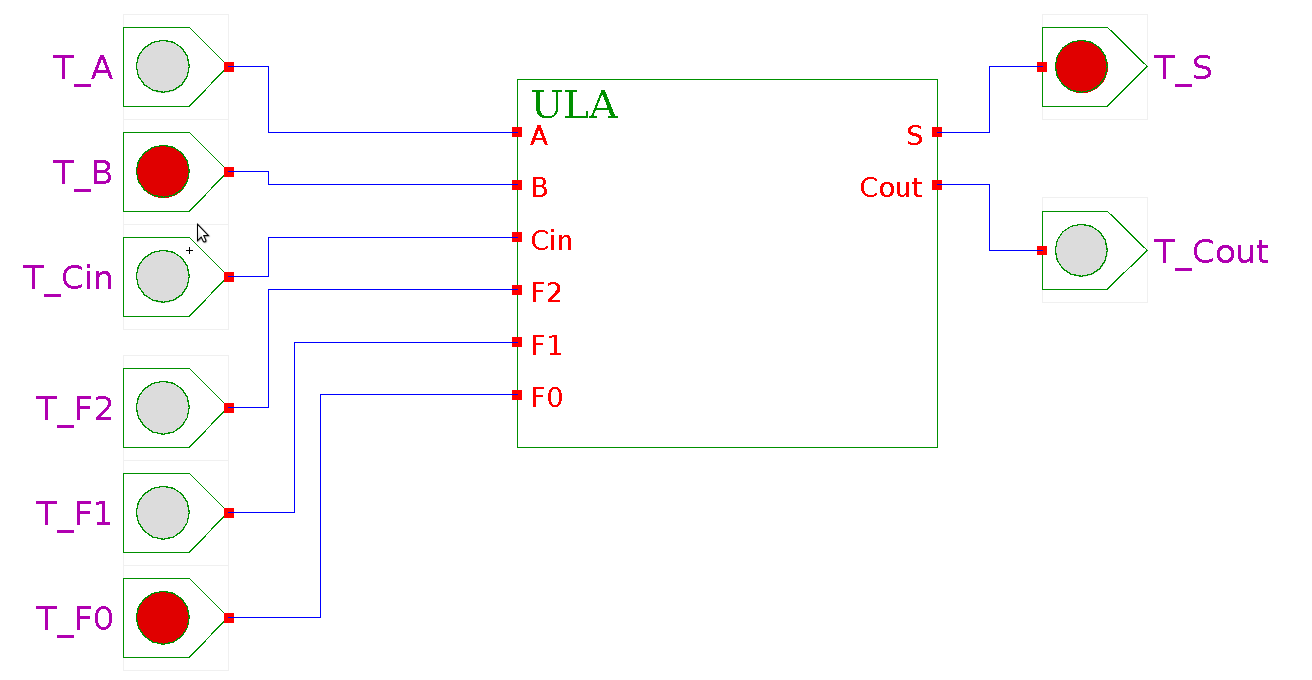
\includegraphics[width=1\textwidth]{figuras/ULA_000.png}
%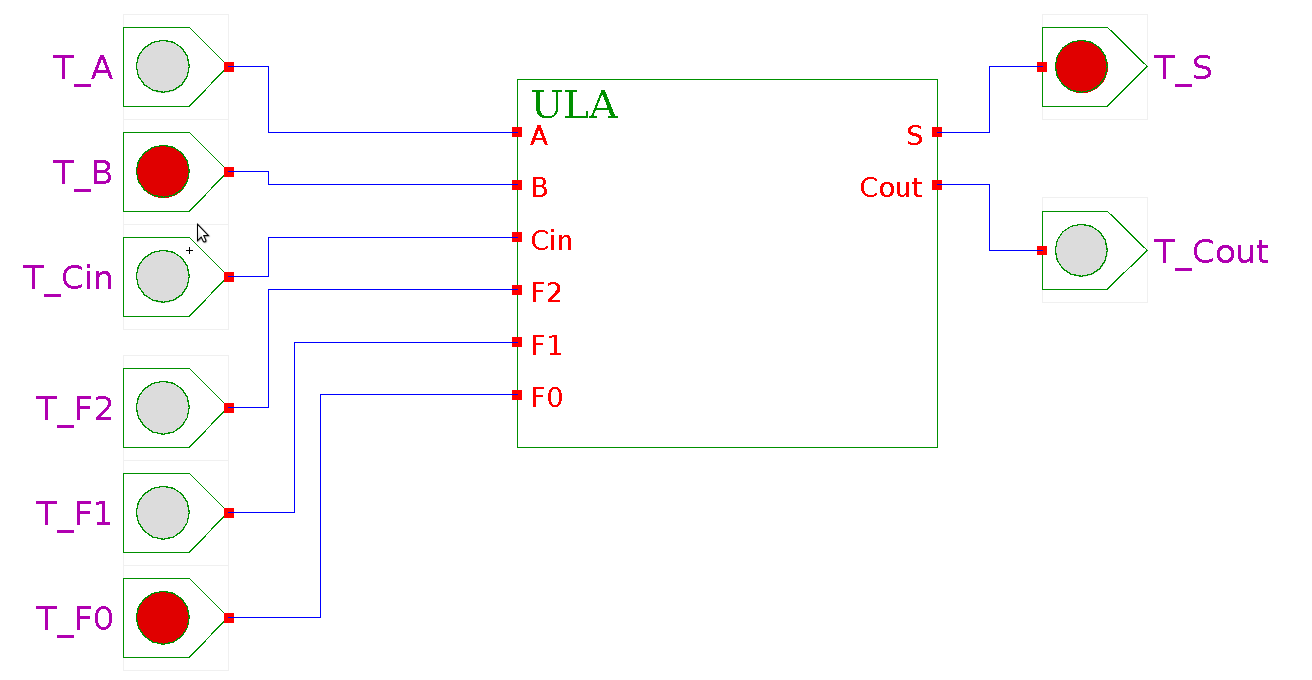
\includegraphics[scale=0.3]{figuras/ULA_000.png}
\caption{Visão da ULA em um nível 0}
\label{fig:ULA_000}
\end{figure}

Em um nível 1, podemos visualizar o detalhamento da ULA, expondo seus componentes, conforme podemos visualizar na Figura~\ref{fig:ULA_001}.

\begin{figure}[H]
\centering
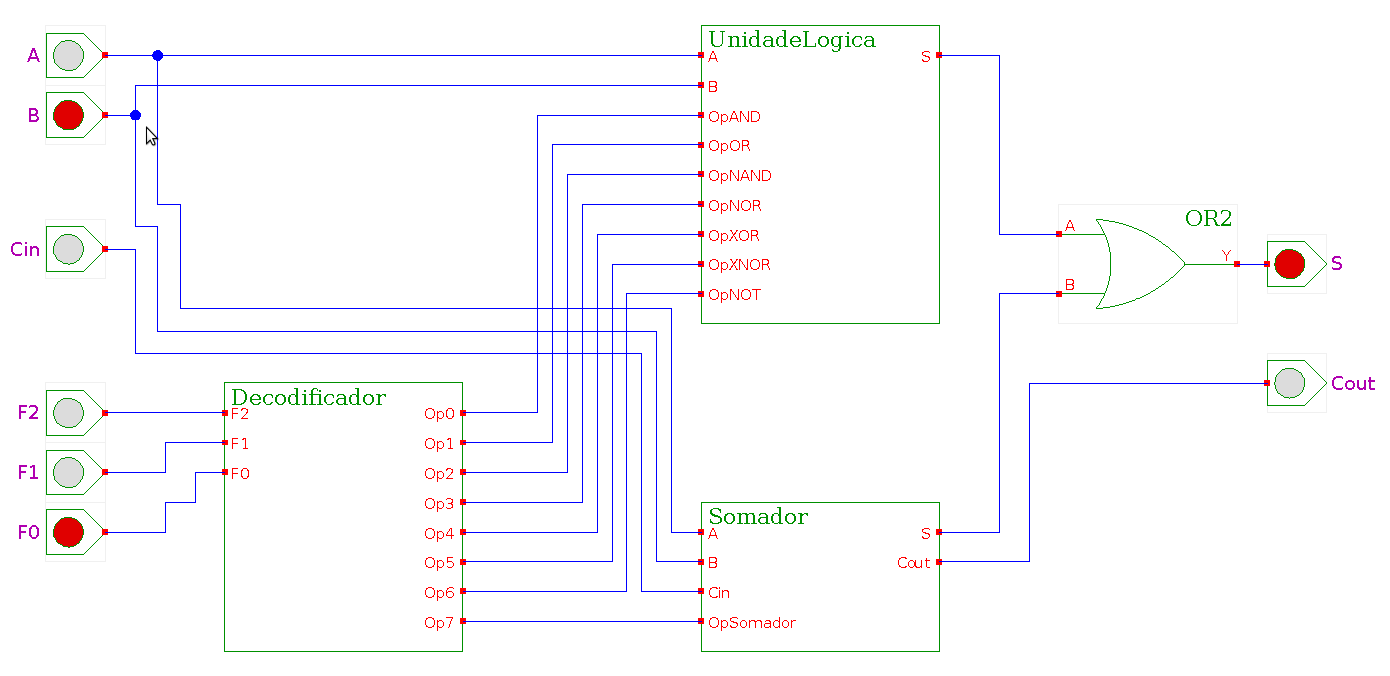
\includegraphics[width=1\textwidth]{figuras/ULA_001.png}
\caption{Visão da ULA em um nível 1, exposição dos componentes principais.}
\label{fig:ULA_001}
\end{figure}


\subsection {Análise e Levantamento de componentes}
Analisando nossa entidade ULA, conforme Figura~\ref{fig:ULA_001}, podemos verificar que a ULA tem um Somador, um Decodificador, uma UnidadeLogica e uma xor2.
O circuito da entidade Somador é apresentado na Figura~\ref{fig:Somador}, podemos ver que realiza a soma das variáveis de entrada A, B e Cin, sendo que Cin é o \emph{Carry} de entrada, o "vai-um" de uma possível coluna anterior.

\begin{figure}[H]
\centering
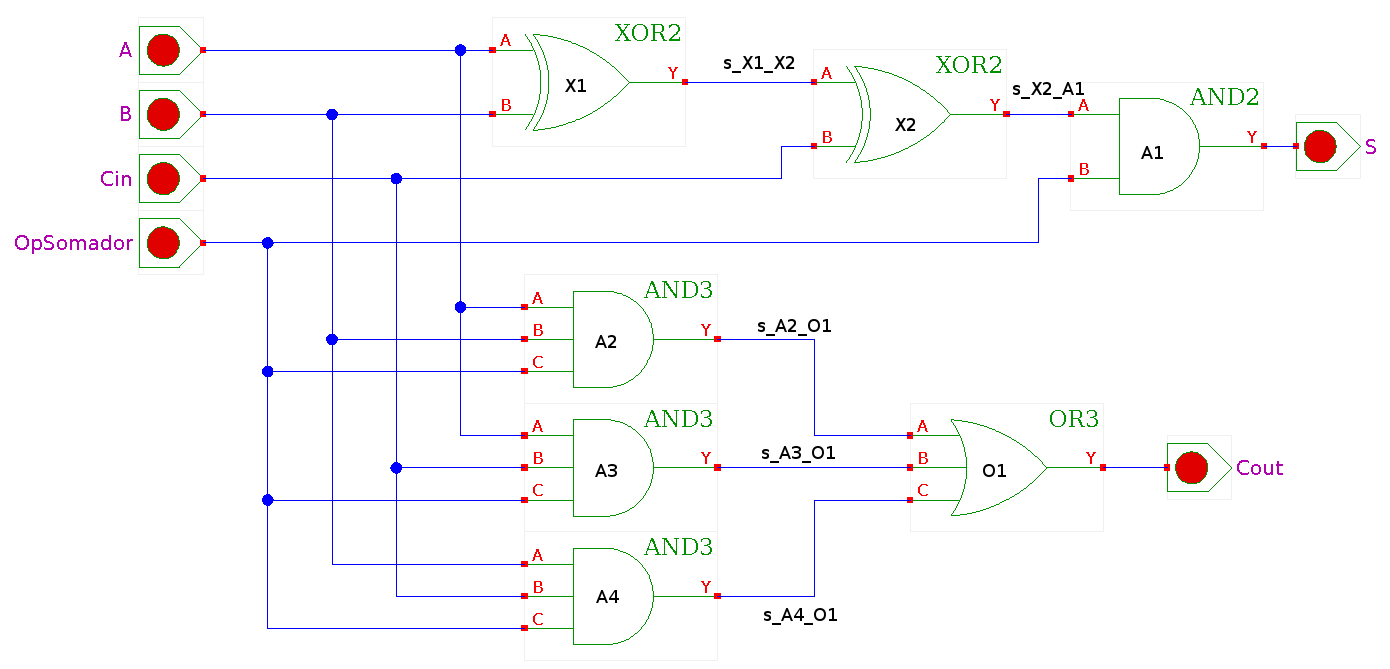
\includegraphics[width=1\textwidth]{figuras/somador.png}
\caption{Circuito Somador.}
\label{fig:Somador}
\end{figure}

O circuito Decodificador é uma circuito para decoficar a operação codificada pela escolha das entradas F\_2, F\_1 e F\_0. O detalhamento da entidade Decodificador é apresentado na Figura~\ref{fig:Decodificador}.

\begin{figure}[H]
\centering
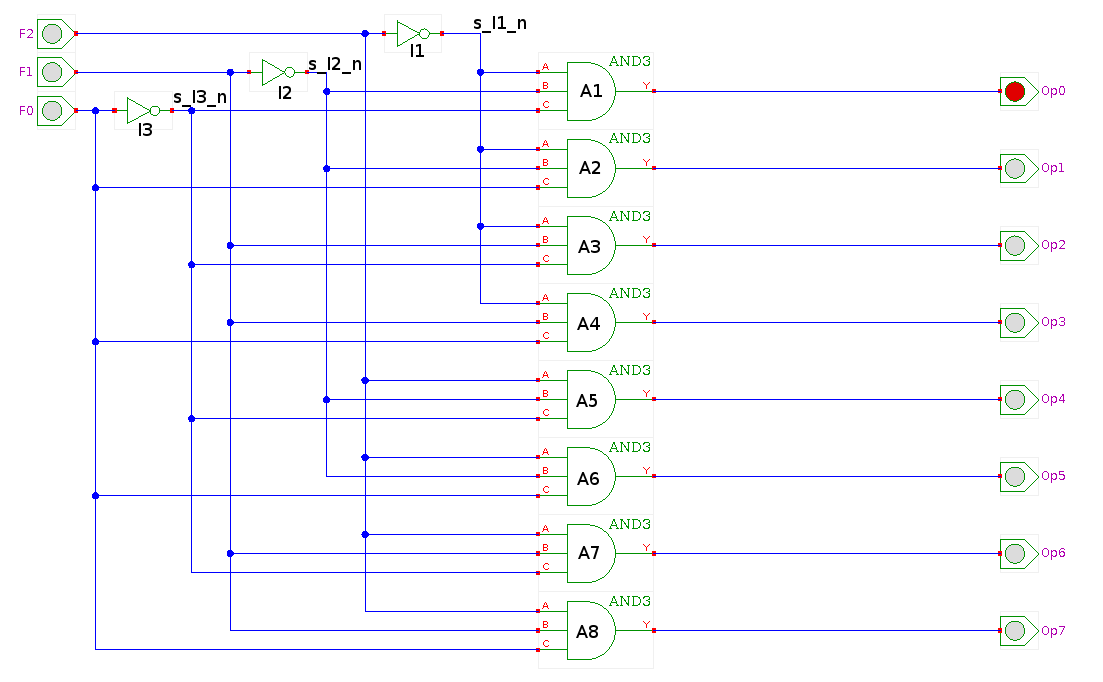
\includegraphics[width=1\textwidth]{figuras/decodificador.png}
\caption{Circuito Decodificador.}
\label{fig:Decodificador}
\end{figure}

As operações suportadas pelo decodificador, consequentemente que são realizadas pela ULA, estão listadas na Tabela~\ref{tab:decod_operacoes}.

\begin{table}[H]
\centering
\caption{Operações suportadas} % igual ao ambiente figura
\begin{tabular}{ccl} % com este comando dizemos quantas colunas terá nossa tabela e a posição do texto dentro de cada coluna. Aqui temos três colunas (pois são três "c" dentre {}) e o texto estará centralizado em todas elas (indicado pelo "c", se quisermos alinhados à esquerda "l" ou direita "r"
\hline % este comando coloca uma linha na tabela
[F\_2][F\_1][F\_0] & Operação & Descrição \\ % esta é a primeira linha de nossa tabela. O símbolo "&" separa as colunas e "\\" indica que aquela linha acabou.
\hline
\hline
000 & Op0 & Operação AND, realizada pela Unidade Lógica. \\
001 & Op1 & Operação OR, realizada pela Unidade Lógica.  \\
010 & Op2 & Operação NAND, realizada pela Unidade Lógica. \\
011 & Op3 & Operação NOR, realizada pela Unidade Lógica.  \\
100 & Op4 & Operação XOR, realizada pela Unidade Lógica.  \\
101 & Op5 & Operação XNOR, realizada pela Unidade Lógica. \\
110 & Op6 & Operação NOT, realizada pela Unidade Lógica.  \\
111 & Op7 & Operação SOMA, realizada pela Somador. \\
\hline
\end{tabular}
\label{tab:decod_operacoes}
\end{table}

As operações suportadas pelo Decodificador de Op0 a Op6 irão selecionar as operações que a Unidade Lógica realiza de OpAND a OpNOT, conforme pode ser visto na Figura~\ref{fig:UnidadeLogica}. O sinal Op7 será ligado ao Somador na entrada OpSomador, entrada que habilita a operação do Somador.

\begin{figure}[H]
\centering
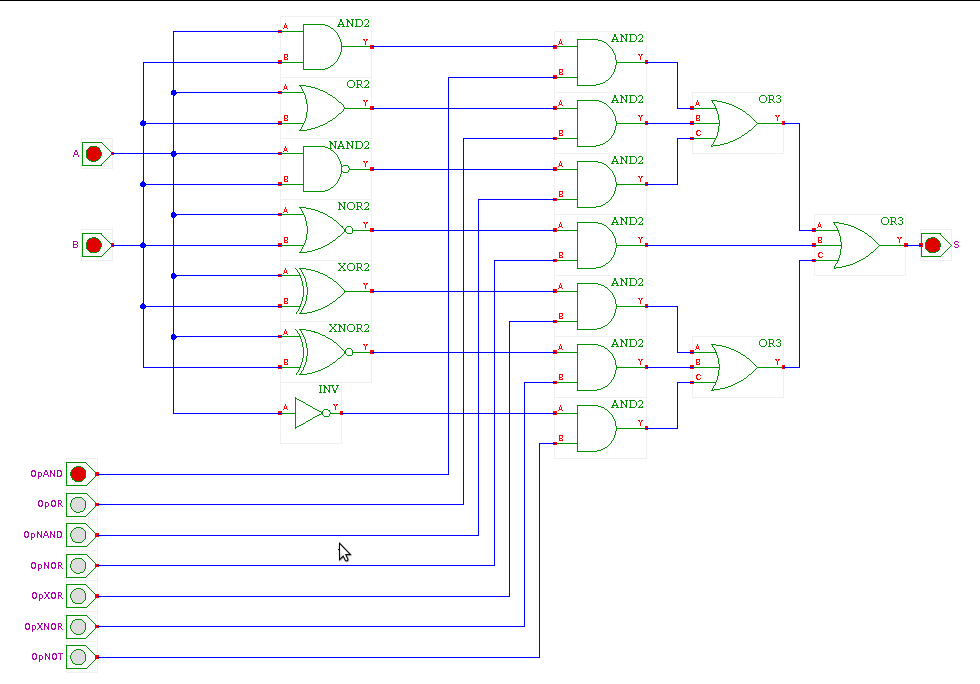
\includegraphics[width=1\textwidth]{figuras/unidadeLogica.png}
\caption{Circuito UnidadeLogica.}
\label{fig:UnidadeLogica}
\end{figure}

Feita essa análise e detalhamento de cada componente, verificamos os subcomponentes de cada componente principal da ULA. Assim, podemos resumir a lista de componentes e suas dependências conforme apresentado na Tabela~\ref{tab:dep_componentes}.

\begin{table}[H]
\centering
\caption{Componentes principais e suas dependências} % igual ao ambiente figura
\begin{tabular}{ll} % com este comando dizemos quantas colunas terá nossa tabela e a posição do texto dentro de cada coluna. Aqui temos três colunas (pois são três "c" dentre {}) e o texto estará centralizado em todas elas (indicado pelo "c", se quisermos alinhados à esquerda "l" ou direita "r"
\hline % este comando coloca uma linha na tabela
Componente & Dependências \\ % esta é a primeira linha de nossa tabela. O símbolo "&" separa as colunas e "\\" indica que aquela linha acabou.
\hline
\hline
ULA & Somador, Decodificador, UnidadeLogica e or2 \\
Somador & xor2, and2, and3 e or3 \\
Decodificador & and3 e inversor \\
UnidadeLogica & or3, and2, or2, nand2, nor2, xor2, xnor2 e inversor \\
\hline
\end{tabular}
\label{tab:dep_componentes}
\end{table} 

\section{Criação dos Componentes com o gcg}

Para satisfazer as dependências da entidade Somador precisamos então criar os componentes básicos, and2, and3, or3 e xor2. O Código~\ref{cod:criar:ent_basicas} apresenta os comandos do Makefile para obter esse resultado. Note que a arquitetura para esses elementos básicos, neste caso portas lógicas, foi definida como lógica, por meio da variável ARCH.

\lstset{numbers=left, numberstyle=\tiny, stepnumber=1, numbersep=3pt}
\begin{lstlisting}[label=cod:criar:ent_basicas,caption=Comandos para a criação das entidades básicas]
  make new PROJECT=and2 ARCH=logica IN=a,b OUT=y
  make new PROJECT=and3 ARCH=logica IN=a,b,c OUT=y
  make new PROJECT=or3 ARCH=logica IN=a,b,c OUT=y
  make new PROJECT=xor2 ARCH=logica IN=a,b OUT=y
\end{lstlisting}

Se verificarmos na estrutura do projeto, foram criados os arquivos das entidades no diretório src e dos testes no diretório testbench. Esse componentes se quisermos fazer o testbench, tudo bem, mas por serem simples portas não precisaria, logo os arquivos dos testbenchs dessas unidades básicas poderiam ser descartados.
O Código~\ref{cod:and2} mostra como o código VHDL para a entidade and2 foi criado pelo make, sendo necessário somente colocarmos o tipo das variáveis e a expressão lógica (y <= a and b) que gera o resultado.

\lstset{language=VHDL}
\lstset{numbers=left, numberstyle=\tiny, stepnumber=1, numbersep=3pt}
\lstinputlisting[label=cod:and2,caption=Código VHDL da entidade and2]{ula/src/and2.vhd}

No diretorio testbench foi criado o arquivo and2\_tb.vhd que é o testbench para a entidade and2, conforme podemos ver no Código~\ref{cod:and2_tb}, novamente alteramos type para std\_logic e criamos os casos de teste.

\lstset{language=VHDL}
\lstset{numbers=left, numberstyle=\tiny, stepnumber=1, numbersep=3pt}
\lstinputlisting[label=cod:and2_tb,caption=Código VHDL do testebench para entidade and2] {ula/testbench/and2_tb.vhd}

Executando o comando make apresentado no Código~\ref{cod:testa:and2}, se tudo estiver correto, a entidade and2 será analisada e compilada e o teste será executado e no final será apresentado a tela do gtkwave com o diagrama de tempo (forma de onda).

\lstset{numbers=left, numberstyle=\tiny, stepnumber=1, numbersep=3pt}
\begin{lstlisting}[label=cod:testa:and2,caption=Comando para executar o testbench da entidade and2.]
  make all TESTBENCH=and2_tb
\end{lstlisting}

O diagrama do resultado pode ser visualizado na Figura~\ref{fig:gtw:and2}.

\begin{figure}[H]
\centering
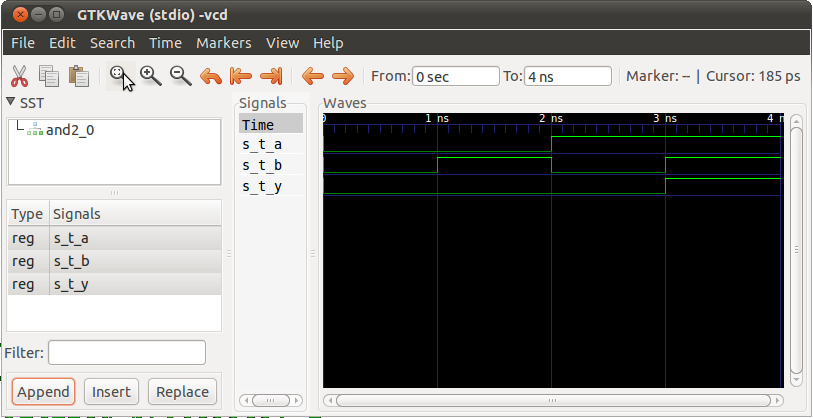
\includegraphics[width=1\textwidth]{figuras/gtw_and2.png}
\caption{Diagrama de Tempo do teste da entidade and2.}
\label{fig:gtw:and2}
\end{figure}

% and3, xor2 e or3
O Código~\ref{cod:and3} mostra o código VHDL para a entidade and3 que foi criado pelo comando make, da mesma forma sendo necessário somente colocarmos o tipo das variáveis e a expressão lógica (y <= a and b and c) para que o resultado seja gerado corretamente.

\lstset{language=VHDL}
\lstset{numbers=left, numberstyle=\tiny, stepnumber=1, numbersep=3pt}
\lstinputlisting[label=cod:and3,caption=Código VHDL da entidade and3]{ula/src/and3.vhd}

No diretorio testbench também foi criado o arquivo and3\_tb.vhd que é o testbench para a entidade and3, conforme podemos ver no Código~\ref{cod:and3_tb}, novamente alteramos <<type>> para std\_logic e criamos os casos de teste.

\lstset{language=VHDL}
\lstset{numbers=left, numberstyle=\tiny, stepnumber=1, numbersep=3pt}
\lstinputlisting[label=cod:and3_tb,caption=Código VHDL do testebench para entidade and3] {ula/testbench/and3_tb.vhd}

Executando o comando make apresentado no Código~\ref{cod:testa:and3}, se tudo estiver correto, a entidade and3 será analisada e compilada e o teste será executado e no final será apresentado a tela do gtkwave com o diagrama de tempo (forma de onda).

\lstset{numbers=left, numberstyle=\tiny, stepnumber=1, numbersep=3pt}
\begin{lstlisting}[label=cod:testa:and3,caption=Comando para executar o testbench da entidade and3.]
  make all TESTBENCH=and3_tb
\end{lstlisting}

O diagrama do resultado pode ser visualizado na Figura~\ref{fig:gtw:and3}.

\begin{figure}[H]
\centering
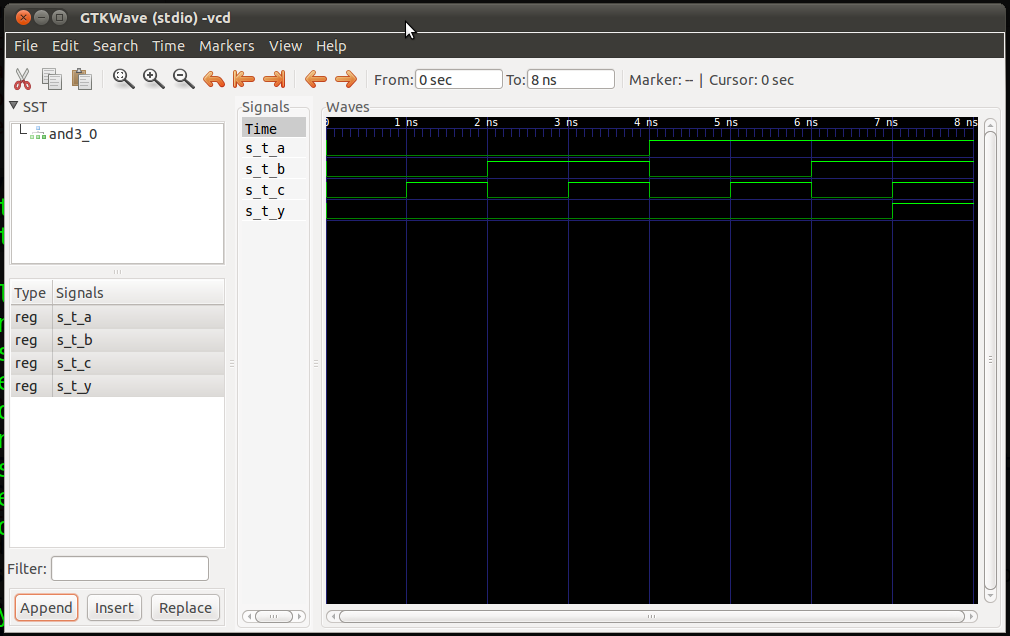
\includegraphics[width=1\textwidth]{figuras/gtw_and3.png}
\caption{Diagrama de Tempo do teste da entidade and3.}
\label{fig:gtw:and3}
\end{figure}

% xor2
O Código~\ref{cod:xor2} mostra o código VHDL para a entidade xor2 que foi criado pelo comando make, da mesma forma sendo necessário somente colocarmos o tipo das variáveis e a expressão lógica (y <= a xor b) para que o resultado seja gerado corretamente.

\lstset{language=VHDL}
\lstset{numbers=left, numberstyle=\tiny, stepnumber=1, numbersep=3pt}
\lstinputlisting[label=cod:xor2,caption=Código VHDL da entidade xor2]{ula/src/xor2.vhd}

No diretorio testbench também foi criado o arquivo xor2\_tb.vhd que é o testbench para a entidade xor2, conforme podemos ver no Código~\ref{cod:xor2_tb}, novamente alteramos <<type>> para std\_logic e criamos os casos de teste.

\lstset{language=VHDL}
\lstset{numbers=left, numberstyle=\tiny, stepnumber=1, numbersep=3pt}
\lstinputlisting[label=cod:xor2_tb,caption=Código VHDL do testebench para entidade xor2] {ula/testbench/xor2_tb.vhd}

Executando o comando make apresentado no Código~\ref{cod:testa:xor2}, se tudo estiver correto, a entidade xor2 será analisada e compilada e o teste será executado e no final será apresentado a tela do gtkwave com o diagrama de tempo (forma de onda).

\lstset{numbers=left, numberstyle=\tiny, stepnumber=1, numbersep=3pt}
\begin{lstlisting}[label=cod:testa:xor2,caption=Comando para executar o testbench da entidade xor2.]
  make all TESTBENCH=xor2_tb
\end{lstlisting}

O diagrama do resultado pode ser visualizado na Figura~\ref{fig:gtw:xor2}.

\begin{figure}[H]
\centering
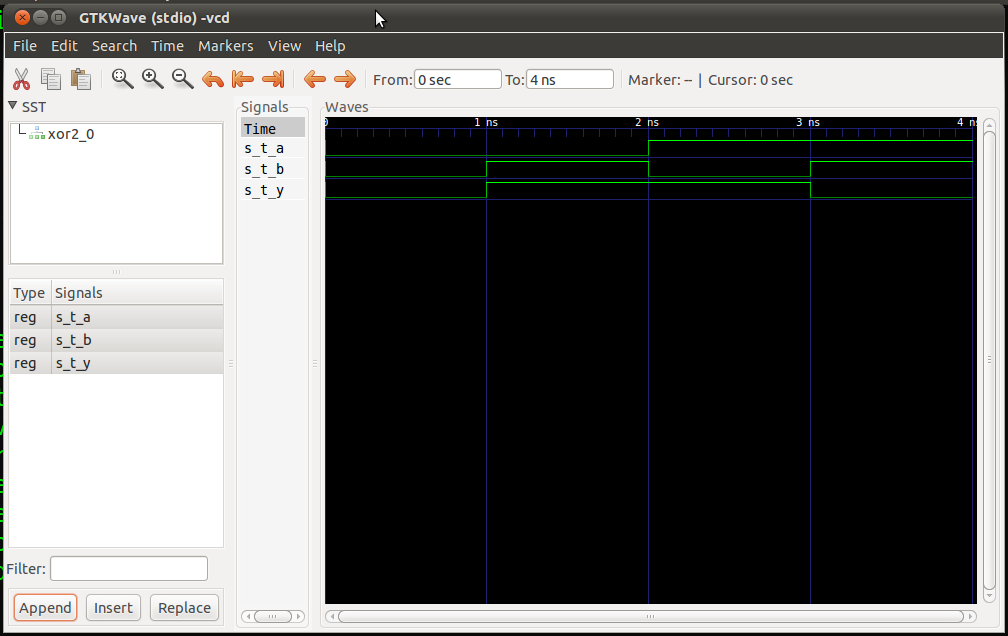
\includegraphics[width=1\textwidth]{figuras/gtw_xor2.png}
\caption{Diagrama de Tempo do teste da entidade xor2.}
\label{fig:gtw:xor2}
\end{figure}

% or3
O Código~\ref{cod:or3} mostra o código VHDL para a entidade or3 que foi criado pelo comando make, da mesma forma sendo necessário somente colocarmos o tipo das variáveis e a expressão lógica (y <= a xor b) para que o resultado seja gerado corretamente.

\lstset{language=VHDL}
\lstset{numbers=left, numberstyle=\tiny, stepnumber=1, numbersep=3pt}
\lstinputlisting[label=cod:or3,caption=Código VHDL da entidade or3]{ula/src/or3.vhd}

No diretorio testbench também foi criado o arquivo or3\_tb.vhd que é o testbench para a entidade or3, conforme podemos ver no Código~\ref{cod:or3_tb}, novamente alteramos <<type>> para std\_logic e criamos os casos de teste.

\lstset{language=VHDL}
\lstset{numbers=left, numberstyle=\tiny, stepnumber=1, numbersep=3pt}
\lstinputlisting[label=cod:or3_tb,caption=Código VHDL do testebench para entidade or3] {ula/testbench/or3_tb.vhd}

Executando o comando make apresentado no Código~\ref{cod:testa:or3}, se tudo estiver correto, a entidade or3 será analisada e compilada e o teste será executado e no final será apresentado a tela do gtkwave com o diagrama de tempo (forma de onda).

\lstset{numbers=left, numberstyle=\tiny, stepnumber=1, numbersep=3pt}
\begin{lstlisting}[label=cod:testa:or3,caption=Comando para executar o testbench da entidade or3.]
  make all TESTBENCH=or3_tb
\end{lstlisting}

O diagrama do resultado pode ser visualizado na Figura~\ref{fig:gtw:or3}.

\begin{figure}[H]
\centering
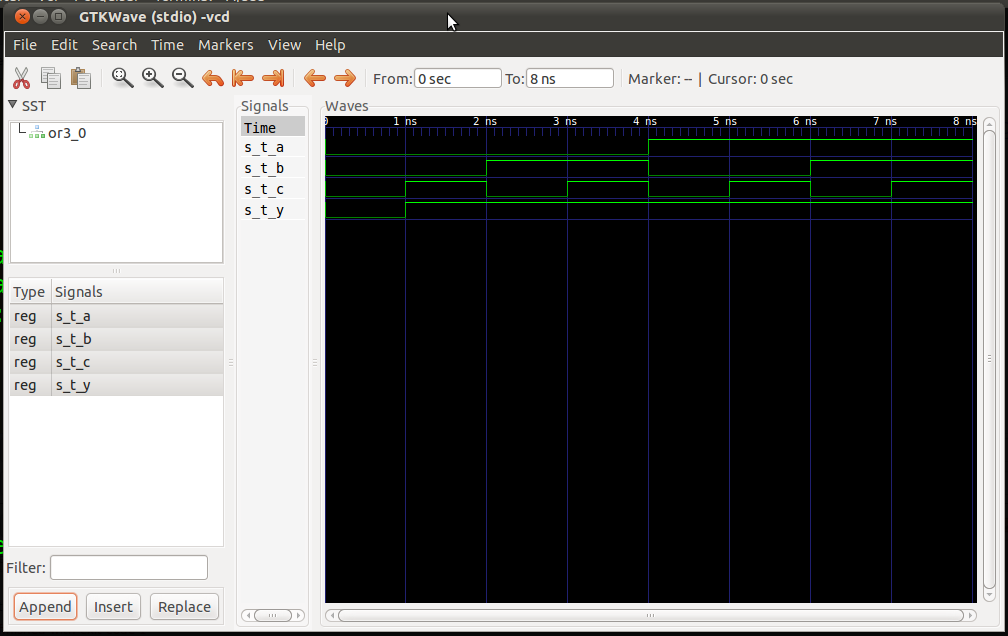
\includegraphics[width=1\textwidth]{figuras/gtw_or3.png}
\caption{Diagrama de Tempo do teste da entidade or3.}
\label{fig:gtw:or3}
\end{figure}

% Somador.
Criadas as entidades básicas necessárias, então podemos criar a entidade principal Somador com o comando apresentado no Código~\ref{cod:criar:somador}. O Somador foi criado com a arquitetura estrutural com o valor da variável ARCH=estrutural.

\lstset{numbers=left, numberstyle=\tiny, stepnumber=1, numbersep=3pt}
\begin{lstlisting}[label=cod:criar:somador,caption=Comando para a criar a entidade Somador.]
  make new PROJECT=somador ARCH=estrutural IN=A,B,Cin,OpSomador OUT=S,Cout
\end{lstlisting}

Criada a entidade Somador apenas é necessário terminar a implementação da arquitetura e do testbench para a entidade.

O Código~\ref{cod:somador} mostra o código VHDL para a entidade somador que foi criado pelo comando make, sendo necessário implementarmos sua função lógica pelo mapeamento das estruturas (port map), já que definimos sua arquitetura como estrutural.

\lstset{language=VHDL}
\lstset{numbers=left, numberstyle=\tiny, stepnumber=1, numbersep=3pt}
\lstinputlisting[label=cod:somador,caption=Código VHDL da entidade somador]{ula/src/somador.vhd}

No diretorio testbench também foi criado o arquivo somador\_tb.vhd que é o testbench para a entidade somador, conforme podemos ver no Código~\ref{cod:somador_tb}, novamente alteramos <<type>> para std\_logic e criamos os casos de teste.

\lstset{language=VHDL}
\lstset{numbers=left, numberstyle=\tiny, stepnumber=1, numbersep=3pt}
\lstinputlisting[label=cod:somador_tb,caption=Código VHDL do testebench para entidade somador] {ula/testbench/somador_tb.vhd}

Executando o comando make apresentado no Código~\ref{cod:testa:somador}, se tudo estiver correto, a entidade somador será analisada e compilada e o teste será executado e no final será apresentado a tela do gtkwave com o diagrama de tempo (forma de onda).

\lstset{numbers=left, numberstyle=\tiny, stepnumber=1, numbersep=3pt}
\begin{lstlisting}[label=cod:testa:somador,caption=Comando para executar o testbench da entidade somador.]
  make all TESTBENCH=somador_tb
\end{lstlisting}

O diagrama do resultado pode ser visualizado na Figura~\ref{fig:gtw:somador}.

\begin{figure}[H]
\centering
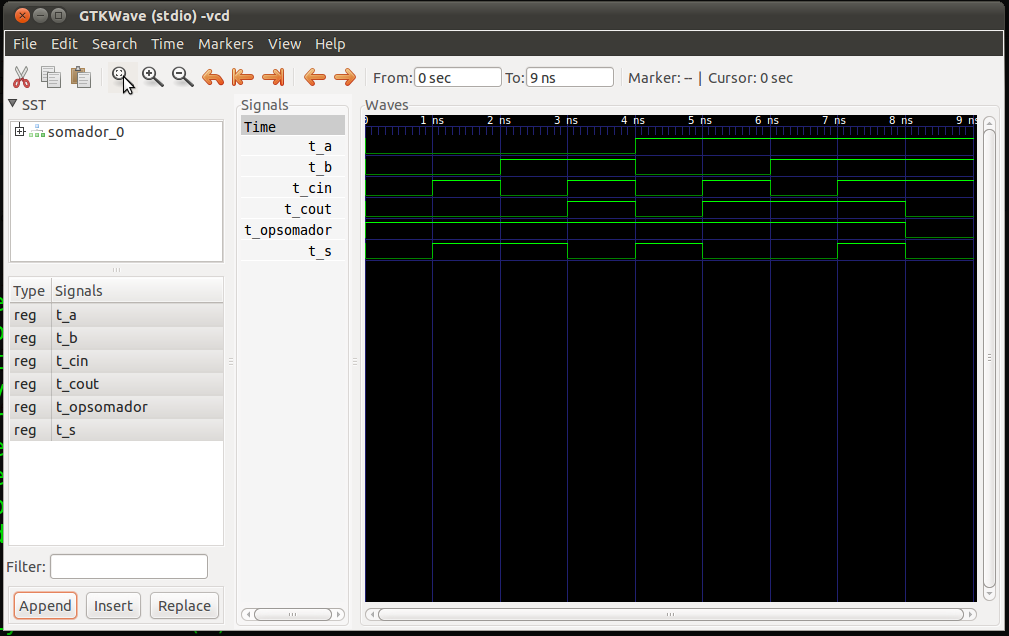
\includegraphics[width=1\textwidth]{figuras/gtw_somador.png}
\caption{Diagrama de Tempo do teste da entidade somador.}
\label{fig:gtw:somador}
\end{figure}

Com o Somador funcionando, podemos ir para a próxima entidade, o Decodificador.
O Decodificador depende de algumas entidades básicas, a maioria já foi criada para satisfazer as dependências da entidade Somador, restando apenas a criação de um inversor, conforme o Código~\ref{cod:criar:inversor}.
% inversor.
\lstset{numbers=left, numberstyle=\tiny, stepnumber=1, numbersep=3pt}
\begin{lstlisting}[label=cod:criar:inversor,caption=Comando para a criar a entidade Inversor.]
  make new PROJECT=inversor ARCH=logica IN=a OUT=y
\end{lstlisting}

O Código~\ref{cod:inversor} mostra o código VHDL para a entidade inversor que foi criado pelo comando make, da mesma forma sendo necessário somente colocarmos o tipo das variáveis e a expressão lógica (y <= not a) para que o resultado seja gerado corretamente.

\lstset{language=VHDL}
\lstset{numbers=left, numberstyle=\tiny, stepnumber=1, numbersep=3pt}
\lstinputlisting[label=cod:inversor,caption=Código VHDL da entidade inversor]{ula/src/inversor.vhd}

No diretorio testbench também foi criado o arquivo inversor\_tb.vhd que é o testbench para a entidade inversor, conforme podemos ver no Código~\ref{cod:inversor_tb}, novamente alteramos <<type>> para std\_logic e criamos os casos de teste.

\lstset{language=VHDL}
\lstset{numbers=left, numberstyle=\tiny, stepnumber=1, numbersep=3pt}
\lstinputlisting[label=cod:inversor_tb,caption=Código VHDL do testebench para entidade inversor] {ula/testbench/inversor_tb.vhd}

Executando o comando make apresentado no Código~\ref{cod:testa:inversor}, se tudo estiver correto, a entidade inversor será analisada e compilada e o teste será executado e no final será apresentado a tela do gtkwave com o diagrama de tempo (forma de onda).

\lstset{numbers=left, numberstyle=\tiny, stepnumber=1, numbersep=3pt}
\begin{lstlisting}[label=cod:testa:inversor,caption=Comando para executar o testbench da entidade inversor.]
  make all TESTBENCH=inversor_tb
\end{lstlisting}

O diagrama do resultado pode ser visualizado na Figura~\ref{fig:gtw:inversor}.

\begin{figure}[H]
\centering
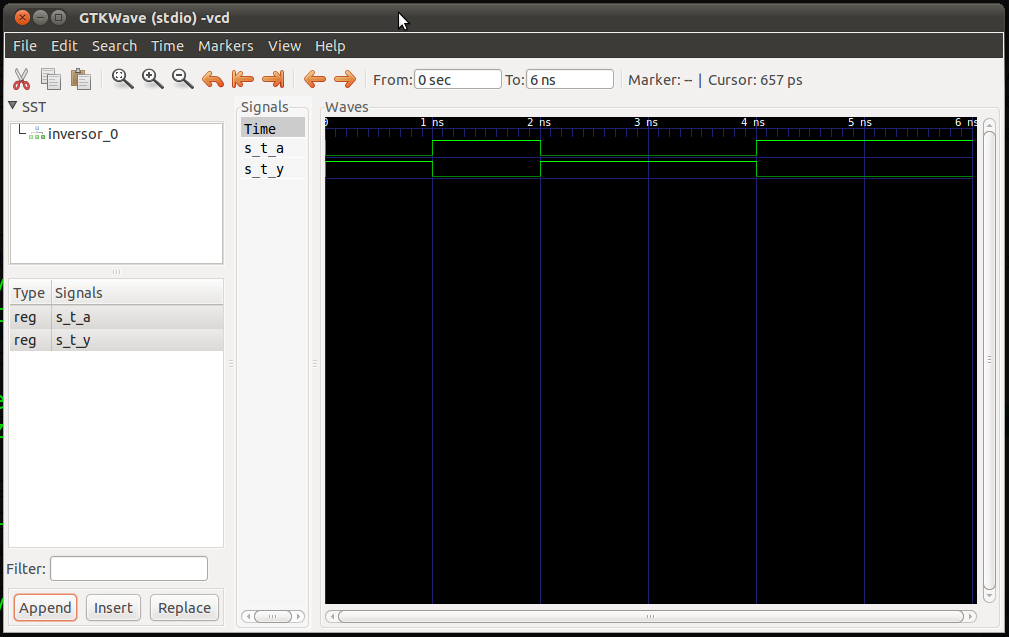
\includegraphics[width=1\textwidth]{figuras/gtw_inversor.png}
\caption{Diagrama de Tempo do teste da entidade inversor.}
\label{fig:gtw:inversor}
\end{figure}

% Decodificador.
Com todas as dependências do Decodificador satisfeitas, podemos então criá-lo, com o comando apresenta no Código~\ref{cod:criar:decodificador}.

\lstset{numbers=left, numberstyle=\tiny, stepnumber=1, numbersep=3pt}
\begin{lstlisting}[label=cod:criar:decodificador,caption=Comando para a criar a entidade Decodificador.]
  make new PROJECT=decodificador ARCH=estrutural IN=F2,F1,F0 OUT=Op0,Op1,Op2,Op3,Op4,Op5,Op6,Op7
\end{lstlisting}

O Código~\ref{cod:decodificador} mostra o código VHDL para a entidade decodificador que foi criado pelo comando make, da mesma forma sendo necessário somente colocarmos o tipo das variáveis e fazer o mapeamento das portas para que o resultado seja gerado corretamente.

\lstset{language=VHDL}
\lstset{numbers=left, numberstyle=\tiny, stepnumber=1, numbersep=3pt}
\lstinputlisting[label=cod:decodificador,caption=Código VHDL da entidade decodificador]{ula/src/decodificador.vhd}

No diretório testbench também foi criado o arquivo decodificador\_tb.vhd que é o testbench para a entidade decodificador, conforme podemos ver no Código~\ref{cod:decodificador_tb}, novamente alteramos <<type>> para std\_logic e criamos os casos de teste.

\lstset{language=VHDL}
\lstset{numbers=left, numberstyle=\tiny, stepnumber=1, numbersep=3pt}
\lstinputlisting[label=cod:decodificador_tb,caption=Código VHDL do testebench para entidade decodificador] {ula/testbench/decodificador_tb.vhd}

Executando o comando make apresentado no Código~\ref{cod:testa:decodificador}, se tudo estiver correto, a entidade decodificador será analisada e compilada e o teste será executado e no final será apresentado a tela do gtkwave com o diagrama de tempo (forma de onda).

\lstset{numbers=left, numberstyle=\tiny, stepnumber=1, numbersep=3pt}
\begin{lstlisting}[label=cod:testa:decodificador,caption=Comando para executar o testbench da entidade decodificador.]
  make all TESTBENCH=decodificador_tb
\end{lstlisting}

O diagrama do resultado pode ser visualizado na Figura~\ref{fig:gtw:decodificador}.

\begin{figure}[H]
\centering
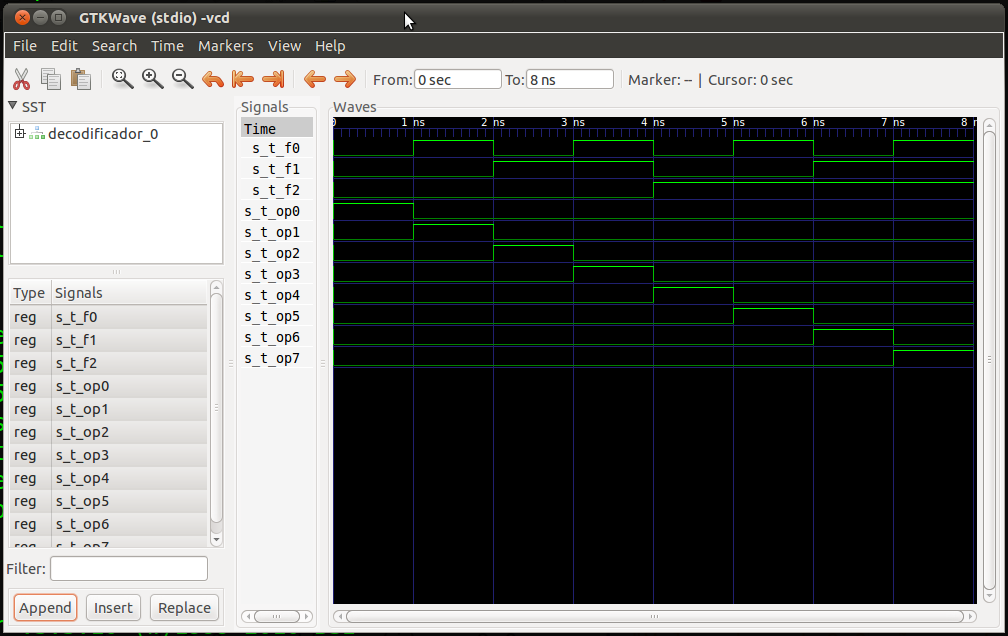
\includegraphics[width=1\textwidth]{figuras/gtw_decodificador.png}
\caption{Diagrama de Tempo do teste da entidade decodificador.}
\label{fig:gtw:decodificador}
\end{figure}

Até implementamos a entidade e testbench do decodificador, deixando-o funcionando.

A próxima entidade a ser criada então é a Unidade Lógica. Para esta entidade precisamos criar os componentes básicos que ainda não temos no projeto e que precisaremos para satisfazer a entidade unidadeLogica, sendo eles or2, nand2, nor2, xnor2. O comando para criá-los é apresentado no Código~\ref{cod:criar:outrasentbasicas}.

\lstset{numbers=left, numberstyle=\tiny, stepnumber=1, numbersep=3pt}
\begin{lstlisting}[label=cod:criar:outrasentbasicas,caption=Comando para a criar entidades básicas para a Unidade Lógica.]
  make new PROJECT=or2 ARCH=logica IN=a,b OUT=y
  make new PROJECT=nand2 ARCH=logica IN=a,b OUT=y
  make new PROJECT=nor2 ARCH=logica IN=a,b OUT=y
  make new PROJECT=xnor2 ARCH=logica IN=a,b OUT=y
\end{lstlisting}

% or2
O Código~\ref{cod:or2} mostra o código VHDL para a entidade or2 que foi criado pelo comando make, da mesma forma sendo necessário somente colocarmos o tipo das variáveis e implementarmos a função lógica (y <= a or b) para que o resultado seja gerado corretamente.

\lstset{language=VHDL}
\lstset{numbers=left, numberstyle=\tiny, stepnumber=1, numbersep=3pt}
\lstinputlisting[label=cod:or2,caption=Código VHDL da entidade or2]{ula/src/or2.vhd}

No diretório testbench também foi criado o arquivo or2\_tb.vhd que é o testbench para a entidade or2, conforme podemos ver no Código~\ref{cod:or2_tb}, novamente alteramos <<type>> para std\_logic e criamos os casos de teste.

\lstset{language=VHDL}
\lstset{numbers=left, numberstyle=\tiny, stepnumber=1, numbersep=3pt}
\lstinputlisting[label=cod:or2_tb,caption=Código VHDL do testebench para entidade or2] {ula/testbench/or2_tb.vhd}

Executando o comando make apresentado no Código~\ref{cod:testa:or2}, se tudo estiver correto, a entidade or2 será analisada e compilada e o teste será executado e no final será apresentado a tela do gtkwave com o diagrama de tempo (forma de onda).

\lstset{numbers=left, numberstyle=\tiny, stepnumber=1, numbersep=3pt}
\begin{lstlisting}[label=cod:testa:or2,caption=Comando para executar o testbench da entidade or2.]
  make all TESTBENCH=or2_tb
\end{lstlisting}

O diagrama do resultado pode ser visualizado na Figura~\ref{fig:gtw:or2}.

\begin{figure}[H]
\centering
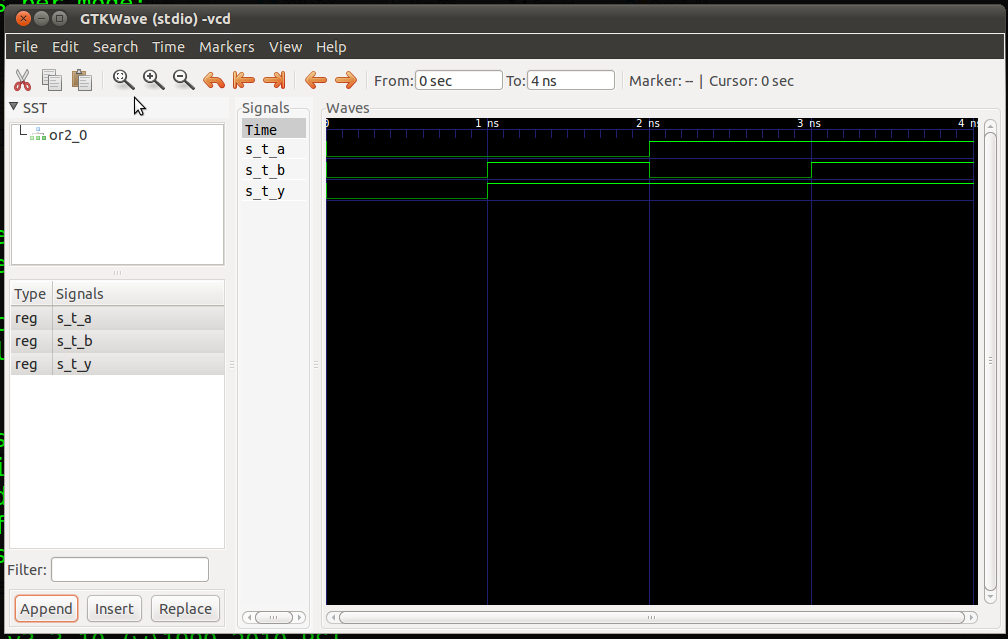
\includegraphics[width=1\textwidth]{figuras/gtw_or2.png}
\caption{Diagrama de Tempo do teste da entidade or2.}
\label{fig:gtw:or2}
\end{figure}

% nand2
O Código~\ref{cod:nand2} mostra o código VHDL para a entidade nand2 que foi criado pelo comando make, da mesma forma sendo necessário somente colocarmos o tipo das variáveis e implementarmos a função lógica (y <= a nand b) para que o resultado seja gerado corretamente.

\lstset{language=VHDL}
\lstset{numbers=left, numberstyle=\tiny, stepnumber=1, numbersep=3pt}
\lstinputlisting[label=cod:nand2,caption=Código VHDL da entidade nand2]{ula/src/nand2.vhd}

No diretório testbench também foi criado o arquivo nand2\_tb.vhd que é o testbench para a entidade nand2, conforme podemos ver no Código~\ref{cod:nand2_tb}, novamente alteramos <<type>> para std\_logic e criamos os casos de teste.

\lstset{language=VHDL}
\lstset{numbers=left, numberstyle=\tiny, stepnumber=1, numbersep=3pt}
\lstinputlisting[label=cod:nand2_tb,caption=Código VHDL do testebench para entidade nand2] {ula/testbench/nand2_tb.vhd}

Executando o comando make apresentado no Código~\ref{cod:testa:nand2}, se tudo estiver correto, a entidade nand2 será analisada e compilada e o teste será executado e no final será apresentado a tela do gtkwave com o diagrama de tempo (forma de onda).

\lstset{numbers=left, numberstyle=\tiny, stepnumber=1, numbersep=3pt}
\begin{lstlisting}[label=cod:testa:nand2,caption=Comando para executar o testbench da entidade nand2.]
  make all TESTBENCH=nand2_tb
\end{lstlisting}

O diagrama do resultado pode ser visualizado na Figura~\ref{fig:gtw:nand2}.

\begin{figure}[H]
\centering
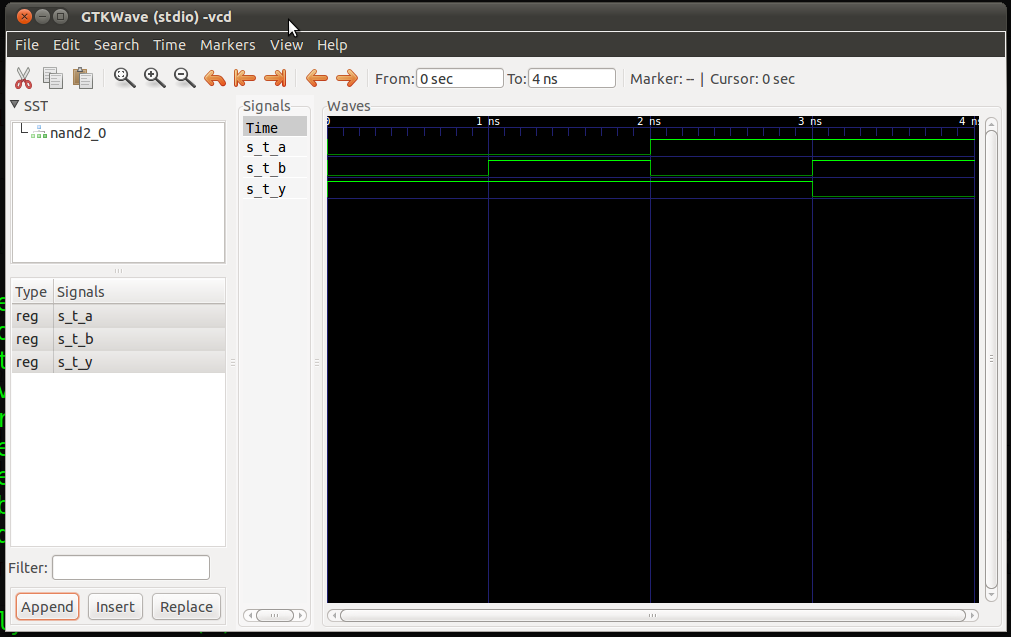
\includegraphics[width=1\textwidth]{figuras/gtw_nand2.png}
\caption{Diagrama de Tempo do teste da entidade nand2.}
\label{fig:gtw:nand2}
\end{figure}
% nor2
O Código~\ref{cod:nor2} mostra o código VHDL para a entidade nor2 que foi criado pelo comando make, da mesma forma sendo necessário somente colocarmos o tipo das variáveis e implementarmos a função lógica (y <= a nor b) para que o resultado seja gerado corretamente.

\lstset{language=VHDL}
\lstset{numbers=left, numberstyle=\tiny, stepnumber=1, numbersep=3pt}
\lstinputlisting[label=cod:nor2,caption=Código VHDL da entidade nor2]{ula/src/nor2.vhd}

No diretório testbench também foi criado o arquivo nor2\_tb.vhd que é o testbench para a entidade nor2, conforme podemos ver no Código~\ref{cod:nor2_tb}, novamente alteramos <<type>> para std\_logic e criamos os casos de teste.

\lstset{language=VHDL}
\lstset{numbers=left, numberstyle=\tiny, stepnumber=1, numbersep=3pt}
\lstinputlisting[label=cod:nor2_tb,caption=Código VHDL do testebench para entidade nor2] {ula/testbench/nor2_tb.vhd}

Executando o comando make apresentado no Código~\ref{cod:testa:nor2}, se tudo estiver correto, a entidade nor2 será analisada e compilada e o teste será executado e no final será apresentado a tela do gtkwave com o diagrama de tempo (forma de onda).

\lstset{numbers=left, numberstyle=\tiny, stepnumber=1, numbersep=3pt}
\begin{lstlisting}[label=cod:testa:nor2,caption=Comando para executar o testbench da entidade nor2.]
  make all TESTBENCH=nor2_tb
\end{lstlisting}

O diagrama do resultado pode ser visualizado na Figura~\ref{fig:gtw:nor2}.

\begin{figure}[H]
\centering
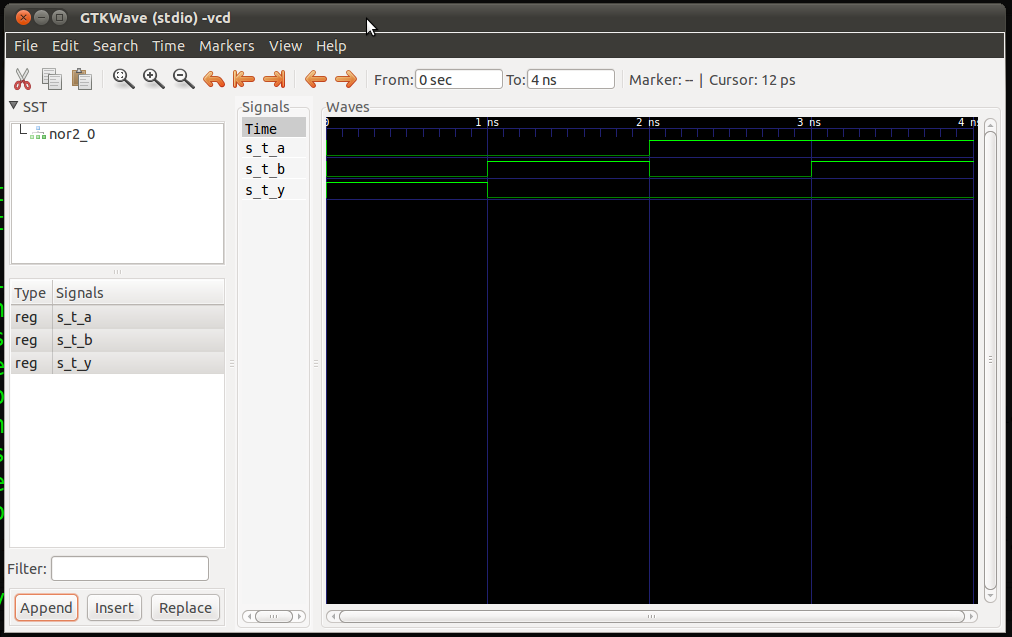
\includegraphics[width=1\textwidth]{figuras/gtw_nor2.png}
\caption{Diagrama de Tempo do teste da entidade nor2.}
\label{fig:gtw:nor2}
\end{figure}

% xnor2
O Código~\ref{cod:xnor2} mostra o código VHDL para a entidade xnor2 que foi criado pelo comando make, da mesma forma sendo necessário somente colocarmos o tipo das variáveis e implementarmos a função lógica (y <= a xor b) para que o resultado seja gerado corretamente.

\lstset{language=VHDL}
\lstset{numbers=left, numberstyle=\tiny, stepnumber=1, numbersep=3pt}
\lstinputlisting[label=cod:xnor2,caption=Código VHDL da entidade xnor2]{ula/src/xnor2.vhd}

No diretório testbench também foi criado o arquivo xnor2\_tb.vhd que é o testbench para a entidade xnor2, conforme podemos ver no Código~\ref{cod:xnor2_tb}, novamente alteramos <<type>> para std\_logic e criamos os casos de teste.

\lstset{language=VHDL}
\lstset{numbers=left, numberstyle=\tiny, stepnumber=1, numbersep=3pt}
\lstinputlisting[label=cod:xnor2_tb,caption=Código VHDL do testebench para entidade xnor2] {ula/testbench/xnor2_tb.vhd}

Executando o comando make apresentado no Código~\ref{cod:testa:xnor2}, se tudo estiver correto, a entidade xnor2 será analisada e compilada e o teste será executado e no final será apresentado a tela do gtkwave com o diagrama de tempo (forma de onda).

\lstset{numbers=left, numberstyle=\tiny, stepnumber=1, numbersep=3pt}
\begin{lstlisting}[label=cod:testa:xnor2,caption=Comando para executar o testbench da entidade xnor2.]
  make all TESTBENCH=xnor2_tb
\end{lstlisting}

O diagrama do resultado pode ser visualizado na Figura~\ref{fig:gtw:xnor2}.

\begin{figure}[H]
\centering
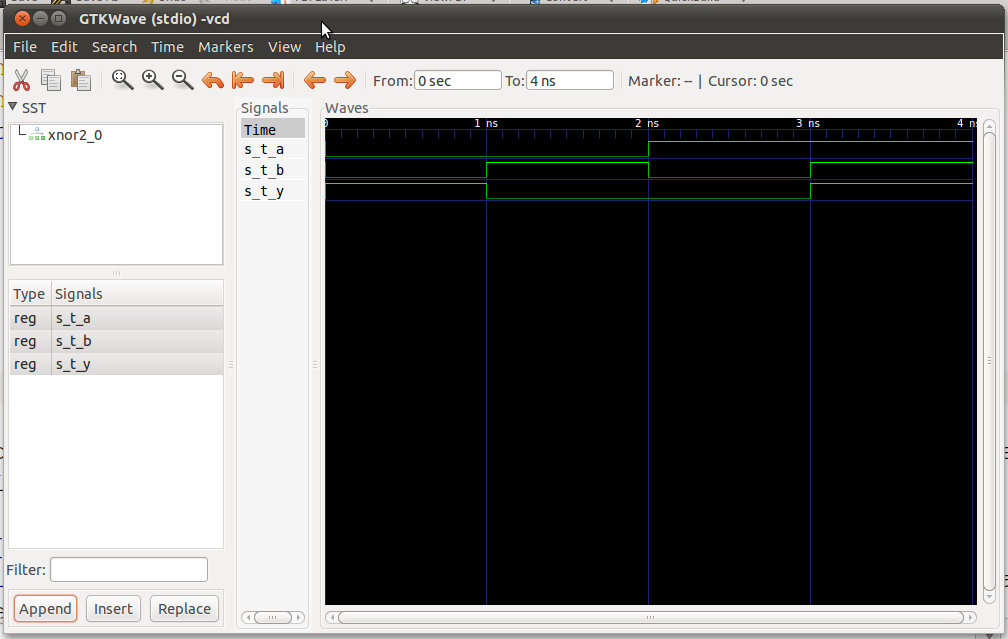
\includegraphics[width=1\textwidth]{figuras/gtw_xnor2.png}
\caption{Diagrama de Tempo do teste da entidade xnor2.}
\label{fig:gtw:xnor2}
\end{figure}

Tendo todas as dependências satisfeitas, podemos então criar a entidade unidadeLogica, conforme o Código~\ref{cod:criar:unidadeLogica}.

\lstset{numbers=left, numberstyle=\tiny, stepnumber=1, numbersep=3pt}
\begin{lstlisting}[label=cod:criar:unidadeLogica,caption=Comando para a criar a entidade unidadeLogica.]
  make new PROJECT=unidadeLogica ARCH=estrutural IN=A,B,OpAND,OpOR,OpNAND,OpNOR,OpXOR,OpXNOR,OpNOT OUT=S
\end{lstlisting}

Implementa-se a entidade e o testbench da unidadeLogica, deixando-a funcionando.

% unidadeLogica

Até aqui, implementamos todos os componentes principais necessários para a implementação da ULA. Então podemos criar a entidade ULA, com o comando apresentado no Código~\ref{cod:criar:ULA}.

\lstset{numbers=left, numberstyle=\tiny, stepnumber=1, numbersep=3pt}
\begin{lstlisting}[label=cod:criar:ULA,caption=Comando para a criar a entidade ULA.]
  make new PROJECT=ula ARCH=estrutural IN=A,B,Cin,F2,F1,F0 OUT=S,Cout
\end{lstlisting}

Verifica-se a implementação da entidade ULA e em seu testbench é necessário apenas a criação dos casos de teste. 

% ULA

Testamos e a deixamos funcionando.
A técnica do menor para o maior, por composição permite ir testando e vendo os resultados dos componentes até atingir o resultado maior que é o projeto como um todo.

Se iniciássemos pela entidade ULA (do maior para o menor) iríamos poder testá-la somente no final, quando todos os componentes estivessem terminados, até lá, muitos erros iriam acontecer.

\end{document}          
